\documentclass{beamer}
\usepackage{graphicx}
\usepackage{amsmath}
\usepackage{xcolor}

\usetheme{Madrid}

\title{Week 10:  Hypothesis Test for Mean and Proportion Parameter}
\author{Kaosar}
\institute{Auburn University}
\date{Spring 2025}

\begin{document}

\begin{frame}
\titlepage
\end{frame}


\begin{frame}{Administrative Items}
\begin{itemize}
    \item Tuesday, April 10: second restricted resource lab
    \item R help
    \item Note sheet updated in each lab
\end{itemize}
\end{frame}






\begin{frame}{Lab Instructions: Step 1 (Set up)}
\begin{itemize}
    \item Install the package:
    \begin{itemize}
        \item \texttt{install.packages("e1071")}
    \end{itemize}
    \item Load the package:
    \begin{itemize}
        \item \texttt{library("e1071")}
    \end{itemize}
    \item To compute skewness of data
\end{itemize}
\end{frame}

\begin{frame}{Types of Skewness}
    \centering
    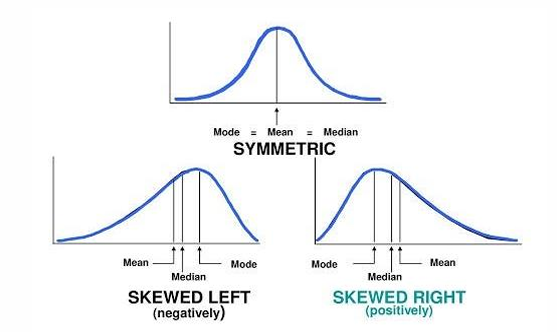
\includegraphics[width=0.8\textwidth]{3611_p9.png}
\end{frame}

\begin{frame}{Lab Instructions: Step 2 (Initial Data Overview)}
\begin{itemize}
    \item Load data:
    \begin{itemize}
        \item \texttt{library("MASS")}
        \item \texttt{data("birthwt")}
    \end{itemize}
    \item Identify column headers:
    \begin{itemize}
        \item \texttt{head(birthwt)}
    \end{itemize}
    \item Number of rows:
    \begin{itemize}
        \item \texttt{nrow(birthwt)}
    \end{itemize}
    \item Add column with birthweight in pounds:
    \begin{itemize}
        \item Example: \texttt{birthwt\$pounds <- birthwt\$bwt / 453.592}
    \end{itemize}
\end{itemize}
\end{frame}

\begin{frame}{Lab Instructions: Step 2 (Continued)}
\begin{itemize}
    \item Create two new data frames:
    \begin{itemize}
        \item Mothers who smoke (=1), mothers who do not smoke (=0)
    \end{itemize}
    \item Compute number of samples, sample mean, variance, and skewness:
    \begin{itemize}
        \item \texttt{nrow()}, \texttt{mean()}, \texttt{var()}, \texttt{skewness()}
    \end{itemize}
\end{itemize}
\end{frame}

\begin{frame}{Lab Instructions: Step 3 (Two-sample t-test)}
\begin{itemize}
    \item Set up plot window: \texttt{par()}
    \item Create QQ plot: \texttt{qqnorm()}
    \item Add reference line:
    \begin{itemize}
        \item Example: \texttt{qqline(data, col = "deeppink", lwd = 2)}
    \end{itemize}
\end{itemize}
\end{frame}

\begin{frame}{Lab Instructions: Step 3 (Two-sample t-test)}
\begin{itemize}
    \item Perform t-test:
    \begin{itemize}
        \item Determine if mean birthweights of two groups are equal
        \item Determine if mean birthweight for smoking mothers $<$ non-smoking mothers
        \item Function: \texttt{t.test()} (use "alternative" argument)
    \end{itemize}
\end{itemize}
\end{frame}

\begin{frame}{Lab Instructions: Step 4 (Hypothesis Test for Proportion)}
\begin{itemize}
    \item Read documentation: \texttt{help(binom.test)} and \texttt{help(prop.test)}
    \item Load precip dataset: \texttt{data("precip")}
    \item Sample size 25:
    \begin{itemize}
        \item \texttt{sample(precip, 25)}
    \end{itemize}
\end{itemize}
\end{frame}

\begin{frame}{Lab Instructions: Step 4 (Continued)}
\begin{itemize}
    \item Hypothesis test (90\% significance):
    \begin{itemize}
        \item Proportion of cities with rainfall $>=$ 20 inches = 0.65
        \item Functions: \texttt{binom.test()}, \texttt{prop.test()}
        \item One-sided test option available
        \item Compute proportion of cities with rainfall $>$ 20 incheses of each year
    \end{itemize}
\end{itemize}
\end{frame}

\begin{frame}{Lab Submissions}
\begin{itemize}
    \item Submit updated note sheet
    \item Submit clearly commented R script
    \item Ensure script runs without errors
    \item Submit Report using Canvas template
    \item Add necessary descriptions or summaries
\end{itemize}
\end{frame}

\end{document}
